% 中文版（Chinese edition）——与 paper/arxiv/main.tex 正文同源，逐段对照翻译。
% 编译：xelatex main && bibtex main && xelatex main && xelatex main
\documentclass[10pt,a4paper,fontset=fandol]{ctexart}
\usepackage[margin=1in]{geometry}
\usepackage{amsmath,amssymb,amsfonts}
\usepackage{graphicx}
\usepackage{booktabs}
\usepackage{multirow}
\usepackage{xcolor}
\usepackage{tikz}
\usetikzlibrary{shapes.geometric,arrows.meta,positioning,fit,calc}
\usepackage[numbers,sort&compress]{natbib}
\usepackage[hidelinks,pdftitle={跨模型规模的缓存翻译：一项带恒等对照与教师内容探针的审计},pdfauthor={Xuemin Zhang, Liangbin Hu, Kun Yi, Liheng Zhong, Junpeng Yu}]{hyperref}

\newcommand{\kv}{\ensuremath{\mathrm{KV}}}
\newcommand{\chg}{\ensuremath{\mathrm{CHG}}}
\newcommand{\gold}{\ensuremath{p_{\mathrm{gold}}}}

\setlength{\emergencystretch}{2em}

\title{跨模型规模的缓存翻译：\\
一项带恒等对照与教师内容探针的审计}

\author{%
Xuemin Zhang\textsuperscript{1}\quad Liangbin Hu\textsuperscript{1}\quad
Kun Yi\textsuperscript{1}\quad Liheng Zhong\textsuperscript{1}\quad
Junpeng Yu\textsuperscript{1}\\[2pt]
\small\texttt{\{zxm0813@gmail.com, huliangbing2000@163.com,}\\
\small\texttt{yikun@bit.edu.cn, lihengzhong@berkeley.edu,
yujunpeng@cetc.com.cn\}}\\[1pt]
\small\textsuperscript{1}CETC
}
\date{}

\begin{document}
\maketitle

\begin{abstract}
跨模型缓存翻译（cache translation）许诺：把大教师模型在上下文上构建的键值
（\kv{}）缓存映射到更小学生模型的缓存空间，从而取消目标侧的预填充
（prefill）。已报告的结果混淆了三个可以各自独立失败的问题：缓存注入流水线是否
忠实保持了一份合法的学生空间缓存（\emph{机制}，mechanics）、映射器能否在替换级
（replacement level）上取代学生自身的缓存（\emph{映射}，mapping）、以及教师
的缓存是否携带冻结学生可以利用的内容（\emph{可利用性}，exploitability）。我们
在严格零 re-prefill 下，对 Qwen3-4B$\to$1.7B 以及另外三个 Qwen3 规模配对
（共四对）同时审计这三者，使用的工具包括逐样本恒等对照、互斥的校准与评测
切分，以及带 bootstrap 区间的金标字母概率指标。机制以数值容差通过：恒等注入
的每个被评测样本相对学生自身 prefill 的 logit 余弦 $\ge 0.9998$（实测最小值
$0.99986$，均值 $0.99998$），变化量为 $+0.0001$ $[-0.0006,+0.0009]$。我们测试
的任何翻译器都没有替换强学生自身的 prefill。审计协议在所有受测配对上记录了
$133$ 个翻译配置；在主要的强学生配对上，最大点估计为 $-0.138$，除最优行
（其区间跨越零）之外，其余区间均位于零以下。对照实验定位了缺口的来源：校准
规模从 $10$ 个样例增加到 $500$ 个只使结果移动 $0.02$；去掉我们最具架构感知的
翻译器的解析锚定会把后缀困惑度从 $501.6$ 降到 $23.7$，而金标变化只移动 $0.045$；
一个 $3700$ 万参数的联合 MLP 也没有帮助。
将我们的实现与最接近的已发表设计对齐——拼接被选中的源层，并在
$1{,}024$~token 的网页文本段上校准——结论不变（$-0.223$ 至 $-0.279$）。弱
$0.6$B 学生达到 $+0.010$ $[-0.089,+0.106]$，这既不能确立退化，也不能确立我们
采用的报告裕度（$\epsilon{=}0.02$）。教师内容探针从未产生区间排除零的增益，
在六个确证性探针配置上的族联合 $95\%$ bootstrap 上界估计为 $+0.009$。审计还给出
两个解耦，我们将其作为支持性证据报告：更好的 \kv{} 重建（留出 $R^2$：键 $0.854$、
值 $0.481$）不改善答案，接近原生的困惑度同样不改善答案。
\end{abstract}

\section{引言}
\label{sec:intro}

服务系统越来越多地在不同模型之间复用计算：同一段长上下文会被多个不同规模的
模型分别预填充。由于 \kv{} 缓存与具体模型绑定，第二个模型通常必须把共享前缀
重新预填充一遍。缓存翻译针对的正是这一点：拟合一个从教师已存储的缓存到学生
缓存空间的映射，之后学生仅凭翻译后的缓存回答一个短查询——即\emph{严格零
re-prefill}~\citep{c2c2025,lsc2026,mot2026,heo2026,cachebridge2026,contextreuse2026}。
已报告的结果目前跨度极大：在 Qwen3 迁移方向上接近原生的保持率
~\citep{cachebridge2026}、在 LongBench2 上超过接收模型自身基线的准确率
~\citep{contextreuse2026}，以及其他设置下的大幅落后。

这一跨度很难解释，因为已发表的评测都是把端到端流水线拿学生基线来打分，从
而混淆了三个可以独立失败的问题：注入流水线是否正确消费了一份外来缓存
（\emph{机制}）？映射是否在替换级上取代了学生自身的缓存（\emph{映射}）？教师
的缓存是否携带冻结学生能够加以利用的内容（\emph{可利用性}）？正向的差值可能
来自这三者中的任何一个，而如果没有把它们分开的仪器，零结果也无法归因。

因此我们把缓存翻译当作一次审计来评测：三条带判定门的假设，每条各配一件
仪器。
\textbf{H1（机制）}：把学生自己的缓存走完整条翻译与注入流水线，应当复现学生
自身的 prefill。
\textbf{H2（映射）}：存在某个受测翻译器达到替换级，以金标字母概率相对学生
自身 prefill 的变化来评分。
\textbf{H3（可利用性）}：受测的教师衍生缓存内容在注入到一份原本原生的学生
缓存中时，能带来增量收益。

我们的贡献是这次审计本身以及它给出的结果，而不是一个新的翻译器。下面三条
结论各自都以我们测试过的设计为界。

\begin{itemize}
\item \textbf{机制不是失效所在。} 恒等对照在数值容差内复现学生（逐样本
logit 余弦均值 $0.99998$，在被评测样本上的最小值 $0.99986$；变化量
$+0.0001$ $[-0.0006,+0.0009]$），并且一对离线/在线运行——在线路径只重新加载
持久化的缓存与映射器——在翻译路径与恒等路径上都与离线结果精确到最后一位
记录数字。
\item \textbf{没有任何受测映射器替换了强学生的缓存。} 线性、逐层、任务感知、
架构锚定与梯度训练的翻译器，从 $10$ 到 $500$ 个样例的校准预算，以及最接近的
已发表设计在其平均形式与拼接形式下的实现，全部失败：强学生配对上的最大点
估计为 $-0.138$ $[-0.312,+0.037]$，其余区间均位于零以下。弱 $0.6$B 学生达到
$+0.010$ $[-0.089,+0.106]$，这既不能确立退化，也不能确立我们的报告裕度。
\item \textbf{没有任何教师内容探针能确立增益。} 把教师衍生内容混入学生自身
的缓存，会随教师占比单调退化；替换顶部三分之一的层是中性的而非有益的；没有
任何探针配置给出在正侧排除零的区间。
\end{itemize}

另外两条结论刻画了否定的锐度；我们把它们作为支持性证据报告，而不是本文的中心。
第一，改善 \kv{} 重建并不改善答案：一个联合 MLP 达到留出 $R^2$ 为 $0.854$（键）
与 $0.481$（值），而逐头仿射映射器为 $0.810$ 与 $0.323$，但它仍然落在同一个 CHG
区间带内。第二，修复困惑度并不修复答案缺口：一个后缀困惑度处在恒等对照的 $2.5$
以内的翻译器，回答正确率为 $26.7\%$，而学生自身为 $50.0\%$。因此在这一设定下，
重建保真度与流畅度都不是任务质量的替代品——同期工作从接收方一侧得出了同一结论
~\citep{cachelink2026}，我们把它视为共有发现，而不是首次报告。

\textbf{适用范围。} 我们测得的是关于所测试设计的一个否定结果，而不是一个
不可能性命题。我们的主配对只涉及一个模型家族，评测是四选一分类，每次运行的
评测样本量 $n$ 在 $10$ 到 $100$ 之间，且报告裕度 $\epsilon$ 是在判定门形式冻结
之后才选定的（第~\ref{sec:framework}~节）。第~\ref{sec:limitations}~节列出了
这留下了哪些开放问题。

\section{相关工作}
\label{sec:survey}

\textbf{单模型内部的 \kv{} 复用。} 提示缓存、缓存增强生成与流式注意力都复用
模型自身的缓存：流式注意力找出了注意力质量异常集中的早期位置
~\citep{streamingsink2023}；CacheGen 压缩并流式传输缓存~\citep{cachegen2024}；
CacheBlend 为检索增强生成融合缓存片段~\citep{cacheblend2025}；KVSharer 在相似
层之间共享缓存~\citep{kvsharer2024}。这些系统假定两侧是同一个模型，因此它们
关心的是存储与注意力开销，而不是表示兼容性。

\textbf{跨模型缓存翻译。} C2C 用按深度比例的层映射直接翻译缓存
~\citep{c2c2025}；LSC 通过共享的隐空间对齐缓存~\citep{lsc2026}；MoT 在按深度
比例的通道窗口上组合门控翻译器，并对上下文做一遍修正
~\citep{mot2026}；KVComm 共享按注意力排序的层~\citep{kvcomm2025}；Interlat
传输最后一层隐状态~\citep{interlat2025}；HCache 从隐状态翻译中恢复缓存
~\citep{hcache2025}。最接近严格零 re-prefill 的设计，从被选中的源层拟合一个
闭式线性映射、对键做去 RoPE，并在匹配 \kv{} 的配对上报告 $73$--$98\%$ 的保持率
~\citep{heo2026}；其非线性变体在两条退化剧烈的配对上能恢复一部分。
两项新近工作进一步拉宽了结果的范围：CacheBridge 保留闭式仿射接口，但把每个
目标头匹配到单一源头，并按注意力敏感度对校准加权~\citep{cachebridge2026}；
一个通用上下文复用层报告说，翻译后的 \kv{} 状态把 Qwen2.5-7B$\to$1.5B 的
LongBench2 准确率从 $27.59\%$ 提升到 $34.48\%$，比接收模型自身的 prefill 高出
$6.89$ 个点~\citep{contextreuse2026}。一项针对混合循环模型的交接研究报告了我们
结论的另一面：仅翻译注意力 \kv{} 与原生行为之间仍留有巨大差距
~\citep{latentport2026}。上述两条引用都在我们冻结之后修订过，因此我们对比的
是它们的设计，而不是它们报告的数字。保持率衡量的是翻译缓存重现接收方自身
prefill 的接近程度，而不是接收方相对自身 prefill 是否有增益，并且这些报告都
没有用恒等对照把机制单独分离出来。
合起来看，已发表的证据如今同时包含接近原生的保持率、高于基线的增益与严重的
退化，这正是需要一个共同审计、而不是支持或反对某个具体翻译器的理由。

\textbf{跨模型表示对齐。} 模型缝合（model stitching）用学到的层连接两个冻结
网络~\citep{stitching2021}；相对表示支持零样本的隐空间通信~\citep{relrep2022}；
柏拉图表示假说及其后续改进主张不同模型之间存在收敛的表示
~\citep{platonic2024,perfectplatonic2025,aristotelian2026}；嵌入空间方法事后对齐
词表~\citep{vec2vec2025}。这一路线支持存在某种共享几何结构，但并未度量该几何
结构是否携带某个具体任务的答案信息。

\textbf{冻结模型的可控性。} 任务向量、激活引导与调好的透镜（tuned lens）表明，
冻结模型的残差流可以被引导或读取
~\citep{taskvectors2023,actsteer2024,tunedlens2023,gist2023}。我们的探针是这些
干预手段在 \kv{} 缓存上的对应物，而它们在我们测试的配对上返回了空结果。FFN
层是键值记忆~\citep{ffnmemory2021}，这也是由权重中介的能力差距未必能以由缓存
中介的形式保留下来的一条理由。

\textbf{这一路线尚未确立什么。} 综观这些工作，没有任何一项被引评测（i）把
机制、映射与可利用性分开，（ii）注入学生自身的缓存作为恒等对照，（iii）在
困惑度匹配的条件下报告准确率，或（iv）用一项无需额外训练的、针对教师衍生
内容的探针来约束可利用性。本次审计提供了这些仪器。

\section{框架}
\label{sec:framework}

\subsection{设定与度量}

教师 $T$ 预填充一段上下文 $x$，并存储缓存
$C_T(x)=\{K^T_\ell,V^T_\ell\}_{\ell=1}^{L_T}$，其中有 $H$ 个 \kv{} 头和头维度
$d$。翻译器 $g_\theta$ 把它映射为学生 $S$ 空间中的 $\widehat C_S(x)$。学生仅凭
$\widehat C_S(x)$ 回答查询 $q$，并且在严格零 re-prefill 下进行：没有任何上下文
token 进入学生的前向计算。每项比较都由三个参照锚定：\emph{学生自 prefill}
$S(q\mid C_S(x))$、把 $C_S(x)$ 送入注入流水线的\emph{恒等注入}，以及\emph{教师
全量 prefill} 参照 $T(q\mid C_T(x))$。

我们用金标字母概率 $\gold$ 来给答案质量打分：它是在最终提示位置上对四个答案
字母 logit 做的 softmax，每个模型使用各自分词器对该字母的 token id。只保留
四选一的样例，因此均匀的四选一预测得分为 $0.25$。全文中的 \emph{CHG} 指在同一批
样例上相对学生自身 prefill 的 $\gold$ 变化，并给出 $95\%$ bootstrap 区间。所有
区间都用评测样例上的配对百分位 bootstrap，重采样 $10^4$ 次，包括
第~\ref{sec:h3}~节中的族联合探针上界。图~\ref{fig:framework} 概括了这一设定与
三件仪器。

\begin{figure}[t]
\centering
% 图 1（中文版）：(a) 被审计的设定，(b) 三个带判定门的问题。
% 与 paper/arxiv/figures/fig1_framework.tex 同构，仅文字改为中文并调整列宽。
% 需在导言区加载：tikz（arrows.meta）、amsmath、amssymb，以及宏 \chg。
\begin{tikzpicture}[
  font=\scriptsize,
  box/.style={draw, rounded corners=2pt, align=center, inner sep=3pt,
              minimum height=8mm, font=\scriptsize},
  tbox/.style={box, fill=blue!8, minimum width=20mm},
  sbox/.style={box, fill=green!10, minimum width=20mm},
  mbox/.style={box, fill=orange!14, minimum width=20mm},
  lab/.style={font=\tiny, align=center},
  flow/.style={-{Latex[length=2mm]}, thick, black!75},
  block/.style={-{Latex[length=2mm]}, thick, dashed, red!75!black},
  ref/.style={-{Latex[length=1.6mm]}, densely dotted, black!55},
  kvk/.style={draw=black!55, fill=blue!18, minimum width=4.6mm,
              minimum height=1.9mm, inner sep=0pt},
  kvv/.style={draw=black!55, fill=orange!28, minimum width=4.6mm,
              minimum height=1.9mm, inner sep=0pt},
]
% ---------------- 面板 (a)：被审计的设定 ----------------
\node[lab, anchor=west] at (-6.3, 2.25) {\textbf{(a)} 被审计的设定};

% 上下文、查询、模型
\node[mbox] (X) at (-5.2, 1.55) {长上下文 $x$};
\node[mbox] (Q) at ( 5.2,-1.45) {查询 $q$};
\node[tbox] (T) at (-5.2, 0) {\textbf{教师} $T$\\冻结};
\node[sbox] (S) at ( 5.2, 0) {\textbf{学生} $S$\\冻结};

% 缓存：逐层的 K/V 堆叠
\foreach \i in {0,1,2}{
  \pgfmathsetmacro{\yy}{0.30-0.30*\i}
  \node[kvk] at (-3.22,\yy) {};
  \node[kvv] at (-2.72,\yy) {};
  \node[kvk] at ( 2.72,\yy) {};
  \node[kvv] at ( 3.22,\yy) {};
}
\node[lab] at (-2.97, 0.68) {$\mathbf{K}$ $\mathbf{V}$};
\node[lab] at (-2.97,-0.80) {$C_T(x)$};
\node[lab] at ( 2.97, 0.68) {$\mathbf{K}$ $\mathbf{V}$};
\node[lab] at ( 2.97,-0.80) {$\hat{C}_S(x)$};

% 翻译器
\node[mbox] (g) at (0, 0) {翻译器 $g_\theta$};
\node[lab] at (0,-0.80) {只读取 $C_T$};

% 穿过缓存的流程
\draw[flow] (T.east) -- (-3.62, 0);
\draw[flow] (-2.32, 0) -- (g.west);
\draw[flow] (g.east) -- (2.32, 0);
\draw[flow] (3.62, 0) -- (S.west);
\draw[flow] (X) -- (T);
\draw[flow] (Q) -- (S);

% 禁止路径：上下文直接进入学生
\draw[block] (X.east) -- (5.2, 1.55) coordinate (turn);
\draw[block] (turn) -- (S.north);
\node[lab] at (0, 2.25)
  {严格零 re-prefill：没有任何上下文的 token 进入学生};
\node[lab, fill=white, inner sep=0.6pt] at (0, 1.55) {\large$\oslash$};

% 参照与度量
\node[lab] at (0,-2.15)
  {基线：学生自 prefill $S(q\mid C_S(x))$ \qquad 参照：
   教师全量 prefill $T(q\mid C_T(x))$};
\node[lab] at (0,-2.85)
  {评分：金标字母概率；\qquad
   $\chg = \mathrm{gold}(\text{交接})-\mathrm{gold}(\text{自 prefill})$};
\end{tikzpicture}

\vspace{1.6mm}
{\footnotesize\textbf{(b)} 三个可以独立失败的问题，每个都有自己的仪器与判定门\par}
\vspace{1.2mm}
{\footnotesize
\setlength{\tabcolsep}{3pt}%
\begin{tabular}{@{}p{0.55cm}p{2.75cm}p{3.35cm}p{3.85cm}p{4.15cm}@{}}
\toprule
 & \textbf{问题} & \textbf{仪器} & \textbf{判定门（固定规则）} & \textbf{结果} \\
\midrule
\textbf{H1} & 注入机制：缓存注入流水线能否无损地保留一份合法的学生空间缓存？
 & 恒等对照：把学生自己的缓存走完整条流水线
 & 每个样本的 logit 余弦 $\ge 0.9998$ $\dagger$
 & 通过：均值 $0.99998$，最小 $0.99986$ \\
\addlinespace[1pt]
\textbf{H2} & 是否有翻译器达到替换级？
 & 翻译器家族；在同一个固定评测集上校准 $10$--$500$
 & $95\%$ CI 下界 $>-\epsilon$，$\epsilon{=}0.02^{\S}$ $\dagger\ddagger$
 & 主配对上未达到（最好 $-0.138$）；两个接近随机的学生
 （三个对齐/未对齐配置）越过该门但无可测增益 \\
\addlinespace[1pt]
\textbf{H3} & 受测的教师衍生内容是否有帮助？
 & 教师内容探针：教师占比、层窗口、八分位；以原生内容作为对照
 & 某个配置的区间在正侧排除 $0$ $\dagger\ddagger$
 & 无 \\
\bottomrule
\end{tabular}}
\par\vspace{1.0mm}
{\tiny $\dagger$ 判定门的形式在运行前固定，其中数值容差在修订期引入
（附录~\ref{app:repro}）；$\S$ $\epsilon{=}0.02$ 是判定门形式冻结之后选定的
报告裕度；$\ddagger$ 冻结判定门扩展。\par}

\caption{被审计的设定与三个带判定门的问题。\textbf{(a)}~教师预填充一段长上下文
并存储其缓存；翻译器把该缓存映射到学生的缓存空间；学生仅凭翻译后的缓存回答
一个短查询，且处于严格零 re-prefill 之下（红色交叉路径）。审计以金标字母概率
相对学生自身 prefill 的变化来衡量这次交接，并以教师的全量 prefill 作为参照点。
\textbf{(b)}~这三个问题可以各自独立失败，因此各自配有自己的仪器与判定门。}
\label{fig:framework}
\end{figure}

\subsection{三条假设、三件仪器、三道判定门}

\textbf{H1（机制）。} 恒等注入逐样本地匹配学生自身的 prefill。\emph{判定门}：
每个被评测样本相对学生自身 prefill 的 logit 余弦 $\ge 0.9998$。该容差与我们
观察到的每一种非恒等方法相差若干数量级，后者的余弦都在 $0.5$ 附近；我们把
实测最小值与判定门一并报告，使该判据可复现，而不是一个等于一的等式。H1 失败
意味着坏掉的是流水线，而不是映射。

\textbf{H2（映射）。} 存在某个受测翻译器达到替换级。\emph{判定门}：CHG 的区间
下界高于 $-\epsilon$，其中 $\epsilon=0.02$ 金标概率——这是一个在判定门形式冻结
之后才选定的\emph{报告裕度}，约为 $0.503$ 学生基线的 $4\%$，并非预先注册的
常数。更严格的增益判定门还要求下界高于 $0$。这一裕度在我们所用的样本量下相当
苛刻：$n{=}30$ 时配对区间的半宽约为 $0.17$，因此 $\epsilon{=}0.02$ 的非劣检验
需要约 $2\times10^{3}$ 个样例。该估计假定真实效应接近零、且方差与已记录的运行
相当；当点估计本身明显低于 $-\epsilon$ 时（例如强学生配对），只要真实效应仍低于
$-\epsilon$，单纯扩大样本量并不能确立非劣。所以我们为每个翻译行报告两个判断，并把
\emph{方向}（上界低于零为\emph{退化}，下界高于零为\emph{增益}，其余为\emph{中性}）
作为推断陈述，\emph{替换}判断并列报告；表~\ref{tab:main} 同时给出两者。

\textbf{H3（可利用性）。} 受测的教师衍生缓存内容在注入到一份原本原生的学生
缓存中时能带来增量收益。\emph{判定门}：存在某个探针配置优于学生自身的缓存，
且其区间在正侧排除零。该探针不新增任何翻译器训练，因此正效应将表明教师衍生内容
在受控干预下是可利用的；而零结果只是在所测试的抽取路径上给出约束，并不排除
所有非线性路径。因此这道判定门针对的是受测内容，而不是教师缓存内在的信息量，
也不针对任何单个映射器的端到端得分。

\subsection{证据等级}
\label{sec:tiers}

这次审计是在修订过程中成长的，因此我们给每一条结论标注它是如何进入协议的。
\emph{确证性}结论在运行之前就已固定：恒等判定门的\emph{形式}（其数值容差
$0.9998$ 是修订期加入的可操作化，附录~\ref{app:repro}）、主配对上的替换判定门
的\emph{形式}与非 $\epsilon$ 的增益判定门，以及按上述规则设定的占比探针与
窗口探针。\emph{冻结判定门扩展}是在修订过程中加入的，并按相同的判定门与度量
评分：残差锚定翻译器与 MLP 翻译器、$8$B 教师、校准阶梯、跨架构与 token 对齐
的学生、$1$K 检索任务、八分位扫描，以及重拟合方差研究。\emph{探索性}分析是
事后从已记录的运行中导出的，措辞上按解释来表述。我们还在
第~\ref{sec:h3}~节报告了对确证性家族的联合 bootstrap，因为没有预先指定更宽
的校正。

\section{方法}
\label{sec:method}

\textbf{模型与配对。} 主配对是 Qwen3-4B（教师）到 Qwen3-1.7B（学生）
~\citep{qwen3}。我们另外在同一协议下运行 Qwen3-4B$\to$Qwen3-0.6B、
Qwen3-8B$\to$Qwen3-1.7B 与 Qwen3-8B$\to$Qwen3-0.6B，以及五个替代学生：
Llama-3.2-1B、Llama-3.2-3B、Gemma-2-2B、Gemma-3-1B 与 Qwen2.5-1.5B。

\textbf{数据。} 校准与评测使用 HellaSwag 与 ARC 的四选一题目，切分互斥。上下文
长度检查使用打包到目标长度的四选一大海捞针（needle-in-a-haystack）任务；
$4$K 与 $8$K 运行以 float16 存储缓存，凡出现这些数字处我们都会标注。

\textbf{协议。} 每个翻译行都在零 re-prefill 下产生，同一次运行中包含恒等对照，
跨模型统一提示格式，对注入的缓存做原生重标定，并逐运行记录 git hash、协议版本
与逐样本得分。上述比较的主评测集是 $100$ 条 HellaSwag/ARC 题目的固定尾部；
映射器阶梯依校准预算使用 $n=30$ 或 $n=63$ 条题目，我们为引用的每个数字都注明
$n$。

\textbf{翻译器。} 我们测试逐头岭回归；逐头仿射（中心化，最强的线性家族）；
逐层仿射；一个任务感知目标；一个由两个模型自身的投影与共享词表对齐构建的
残差锚定翻译器（RAT），并对其组件做消融；一个逐头 MLP；以及一个约 $3700$ 万
参数的逐位置联合 MLP。对最接近的已发表设计，我们实现带去 RoPE 键的 top-$k$
源层选择~\citep{heo2026} 的两种形式：用 $200$ 个审计上下文对被选层取平均，以及
用来自生成式网页文本风格语料的 $100$ 条 $1{,}024$~token 校准序列对被选层做拼接；
参考实现使用 $500$ 条序列（附录~\ref{app:impl}）。

\textbf{校准阶梯。} 对最强的线性家族，我们在同一个固定评测集上把校准预算取为
$10/30/60/100/200/500$ 个样例，使预算效应不会与评测题目相混淆。

\textbf{探针。} 占比探针注入 $\alpha\widehat C_S+(1-\alpha)C_S$，其中
$\alpha\in\{0.25,0.5,0.75\}$；窗口探针用翻译内容替换学生层的底部、中部或顶部
三分之一；八分位探针替换八个层窗口之一。所有探针都需要学生自身的 prefill，
因此它们是测量仪器，而不是可部署系统。

\textbf{诊断。} 我们用与每个家族相同的拟合预算（$20$ 个校准上下文、$10$ 个互斥
留出上下文），度量从教师状态恢复学生自身 $K$ 与 $V$ 的留出重建 $R^2$，并报告
教师与学生之间的 \kv{} 范数比。

\section{结果}
\label{sec:results}

\subsection{H1：机制不是失效所在}
\label{sec:h1}

恒等注入复现了学生自身的 prefill：在主配对上，变化量为 $+0.0001$
$[-0.0006,+0.0009]$，逐样本 logit 余弦平均为 $0.99998$、最差为 $0.99986$
（$n{=}30$），并且该对照在我们报告的每一次其他运行中都成立，其平均余弦位于
$0.99998$ 到 $0.99999$ 之间。这一保证在持久化之后同样成立：一次在线运行只
重新加载持久化的缓存与映射器、从不加载教师，却在记录精度上复现了离线的翻译
结果与恒等结果（$-0.1376$ 与 $+0.00013$）。原生缓存消融在两次运行之间不同，
因为在线路径不携带原生缓存，因此我们把等价性限定在翻译路径与恒等路径上。
于是下文任何缺口都可归因于映射，或归因于它搬运的内容。

\subsection{H2：没有任何受测映射器替换强学生的缓存}
\label{sec:h2}

表~\ref{tab:main} 汇总了映射器阶梯。在四选一分类设定下，相对学生自身 prefill，每个
强学生翻译都有负的点估计，从 $-0.138$ 到 $-0.392$；第~\ref{sec:analysis}~节的长上下文
行在同一对上达到 $-0.596$。除最优配置之外都统计上退化。最优配置
（逐头仿射，$c{=}30$）是唯一一个区间触及零的配置（$-0.138$
$[-0.312,+0.037]$），而它也没有通过替换判定门。三项对照表明，这不是我们实现
选择造成的假象。

\emph{在所测试的范围内，校准规模并不能弥合缺口。} 在一个固定评测集上，同一
家族在六个预算之间移动于 $-0.2569$ 与 $-0.2378$ 之间，对整个区间宽度
$\ge 0.2$ 而言，这只是 $0.02$ 的散布。

\emph{在所测试的范围内，容量与锚定也不能弥合缺口。} 一个逐头 MLP（五次训练，
范围 $-0.39$ 至 $-0.26$）与一个 $3700$ 万参数的联合 MLP（五次训练，$-0.30$ 至
$-0.26$）都落在该线性带内。去掉 RAT 的解析锚定会同时改善两项测量，但幅度悬殊：
后缀困惑度从 $501.6$ 降到 $23.7$，即二十一分之一，而 CHG 只从 $-0.268$ 移到
$-0.223$。流畅度便宜、作答不便宜，这正是第~\ref{sec:analysis}~节要回到的图样；
附录~\ref{app:heo-mlp} 讨论最接近的已发表设计所报告的非线性结果。

\emph{在所测试的范围内，源层组合也不能弥合缺口。} 最接近的已发表设计在我们
能够对齐的两种形式上都失败——它的源层组合与它的序列长度——差别在于校准规模与
语料（附录~\ref{app:impl}）：对被选中的 top-$k$ 层取平均，在 $k{=}1,3,5$ 时
分别给出 $-0.273$、$-0.308$ 与 $-0.291$；用长序列网页文本校准对它们做拼接，
分别给出 $-0.279$、$-0.223$ 与 $-0.254$。六个区间全部位于零以下，且六次运行中
恒等对照全部通过。

\emph{弱学生是另一回事，但也不是正面结果。} 它达到 $+0.010$
$[-0.089,+0.106]$，其区间同时跨越零与 $-\epsilon$：我们既不能确立替换，也不能
确立退化。另外两个弱学生行表现相同（$8$B 教师下为 $-0.023$
$[-0.106,+0.060]$；RAT 为 $-0.041$ $[-0.124,+0.038]$）。在翻译配置中最大的点估计
是 $+0.010$，它属于这一配对；附录~\ref{app:extra} 中的探索性八分层探针含有更大的
正点估计，但没有任何一个确立显著增益。

\begin{table}[t]
\centering
\caption{映射器阶梯（除特别注明外均在主配对上）。Acc/Gold/PPL：翻译缓存的
答案准确率、金标字母概率与后缀困惑度；学生自 prefill 行的困惑度是在完整上下文
上测得的，不可直接比较。CHG 是相对学生自身 prefill 的金标概率变化，带 $95\%$
bootstrap 区间；范围来自相互独立的多次训练。\emph{替换}是
第~\ref{sec:framework}~节的替换判断（当且仅当区间下界高于 $-\epsilon$ 时通过，
$\epsilon{=}0.02$）。\emph{方向}为方向判断（当且仅当区间上界低于零时为
\emph{退化}，下界高于零时为\emph{增益}，其余为\emph{中性}）。两个判断相互独立，
因此一行可以在实践上非劣、同时又在统计上显著差于基线。恒等行由 H1 判定门评分。
$n$ 是评测样本数。标记为 $^{\ddagger}$ 的行是冻结判定门扩展；$^{\sharp}$ 表示
拼接被选中的源层并在 $1{,}024$~token 的网页文本段上校准。}
\label{tab:main}
\resizebox{\columnwidth}{!}{%
\setlength{\tabcolsep}{4pt}
\begin{tabular}{lccccl}
\toprule
配置 & Acc / Gold / PPL & 金标 CHG [95\% CI] & $n$ & 替换 & 方向 \\
\midrule
恒等对照（self-\kv），1.7B & 0.500 / 0.503 / 21.2 & $+0.0001$ [$-0.0006, +0.0009$] & 30 & 通过 & 中性 \\
学生自 prefill，1.7B & 0.500 / 0.503 / 25.4 & -- & 30 & -- & -- \\
教师（Qwen3-4B）完整 prefill & 0.767 / 0.693 / -- & -- & 30 & -- & -- \\
原生缓存注入，1.7B & 0.167 / 0.169 / $5.4\times10^{5}$ & $-0.334$ [$-0.510, -0.149$] & 30 & 不通过 & 退化 \\
岭回归逐头，c30，1.7B & 0.200 / 0.207 / 88.5 & $-0.296$ [$-0.470, -0.112$] & 30 & 不通过 & 退化 \\
仿射逐头，c30，1.7B & 0.367 / 0.365 / 46.1 & $-0.138$ [$-0.312, +0.037$] & 30 & 不通过 & 中性 \\
仿射逐头，c200，1.7B & 0.254 / 0.258 / 56.4 & $-0.239$ [$-0.353, -0.122$] & 63 & 不通过 & 退化 \\
仿射逐层，c200，1.7B & 0.206 / 0.222 / $8.1\times10^{4}$ & $-0.275$ [$-0.404, -0.140$] & 63 & 不通过 & 退化 \\
任务感知，c200，1.7B & 0.270 / 0.280 / 142.1 & $-0.216$ [$-0.336, -0.093$] & 63 & 不通过 & 退化 \\
RAT，c30，1.7B$^{\ddagger}$ & 0.233 / 0.235 / 501.6 & $-0.268$ [$-0.439, -0.092$] & 30 & 不通过 & 退化 \\
RAT，c200，1.7B$^{\ddagger}$ & 0.238 / 0.276 / 1008.2 & $-0.221$ [$-0.342, -0.099$] & 63 & 不通过 & 退化 \\
RAT 无锚定 rank-32，c30$^{\ddagger}$ & 0.267 / 0.280 / 23.7 & $-0.223$ [$-0.369, -0.086$] & 30 & 不通过 & 退化 \\
逐头 MLP，c30（5 次训练）$^{\ddagger}$ & 0.133--0.267 / 0.111--0.246 / 65--96 & $-0.39$ 至 $-0.26$ & 30 & 不通过 & 退化 \\
逐头 MLP，c200（5 次训练）$^{\ddagger}$ & 0.175--0.302 / 0.241--0.271 / 109--149 & $-0.26$ 至 $-0.23$ & 63 & 不通过 & 退化 \\
联合 MLP，c30（5 次训练）$^{\ddagger}$ & 0.167--0.233 / 0.201--0.239 / 26--32 & $-0.30$ 至 $-0.26$ & 30 & 不通过 & 退化 \\
Top-$k$ 岭回归（平均），c200，$k{=}1$$^{\ddagger}$ & 0.240 / 0.238 / 78.5 & $-0.273$ [$-0.386, -0.159$] & 100 & 不通过 & 退化 \\
Top-$k$ 岭回归（平均），c200，$k{=}3$$^{\ddagger}$ & 0.190 / 0.203 / 2630 & $-0.308$ [$-0.414, -0.199$] & 100 & 不通过 & 退化 \\
Top-$k$ 岭回归（平均），c200，$k{=}5$$^{\ddagger}$ & 0.210 / 0.220 / $6.9\times10^{4}$ & $-0.291$ [$-0.396, -0.184$] & 100 & 不通过 & 退化 \\
Top-$k$ 岭回归（拼接，网页文本），$k{=}1$$^{\sharp}$ & 0.230 / 0.233 / $1.6\times10^{5}$ & $-0.279$ [$-0.407, -0.148$] & 100 & 不通过 & 退化 \\
Top-$k$ 岭回归（拼接，网页文本），$k{=}3$$^{\sharp}$ & 0.290 / 0.289 / $4.6\times10^{4}$ & $-0.223$ [$-0.364, -0.081$] & 100 & 不通过 & 退化 \\
Top-$k$ 岭回归（拼接，网页文本），$k{=}5$$^{\sharp}$ & 0.270 / 0.257 / 3678 & $-0.254$ [$-0.391, -0.117$] & 100 & 不通过 & 退化 \\
岭回归逐头，c500，8B$\to$1.7B$^{\ddagger}$ & 0.310 / 0.288 / 146.1 & $-0.224$ [$-0.327, -0.122$] & 100 & 不通过 & 退化 \\
仿射逐头，c200，4B$\to$0.6B & 0.302 / 0.283 / 71.8 & $+0.010$ [$-0.089, +0.106$] & 63 & 不通过 & 中性 \\
仿射逐头，c30，8B$\to$0.6B$^{\ddagger}$ & 0.270 / 0.269 / 99.0 & $-0.023$ [$-0.106, +0.060$] & 100 & 不通过 & 中性 \\
RAT，c200，4B$\to$0.6B$^{\ddagger}$ & 0.206 / 0.232 / 790.0 & $-0.041$ [$-0.124, +0.038$] & 63 & 不通过 & 中性 \\
仿射逐头，c30，1K 检索$^{\ddagger}$ & 0.233 / 0.232 / 6554 & $-0.285$ [$-0.549, -0.003$] & 30 & 不通过 & 退化 \\
仿射逐头，c10，4K 检索$^{\ddagger}$ & 0.200 / 0.200 / $1.6\times10^{4}$ & $-0.596$ [$-0.939, -0.135$] & 10 & 不通过 & 退化 \\
仿射逐头，c10，8K 检索$^{\ddagger}$ & 0.200 / 0.203 / $2.4\times10^{4}$ & $-0.577$ [$-0.943, -0.082$] & 10 & 不通过 & 退化 \\
\bottomrule
\end{tabular}}
\end{table}

\begin{figure}[t]
\centering
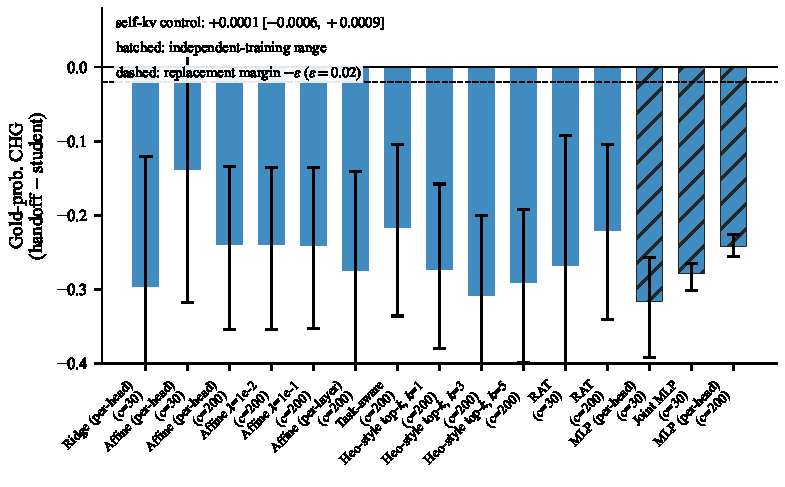
\includegraphics[width=0.95\textwidth]{figures/fig2_mapper_landscape.pdf}
\caption{主配对上的映射器全景：相对学生自身 prefill 的金标字母概率变化与
$95\%$ bootstrap 区间，每个配置一根柱。所有点估计都是负的；其中最优的一个
（逐头仿射在 $c{=}30$）是唯一一个区间触及零的。在校准阶梯上，仿射的估计总共
只移动 $0.02$（表~\ref{tab:main}），而架构锚定、梯度训练与过参数化的翻译器都
落在同一个带内。最接近的已发表设计的长序列拼接变体在表~\ref{tab:main} 中报告，
为便于阅读此处省略。}
\label{fig:landscape}
\end{figure}

\subsection{H3：没有任何教师内容探针能确立增益}
\label{sec:h3}

附录表~\ref{tab:probes} 报告了确证性翻译器（RAT，$c{=}30$）下的探针，以及在
最强线性翻译器（仿射，$c{=}30$）下的复现。

在两种翻译器下，占比探针都随教师占比单调退化，因此在学生自身的缓存中加入
教师衍生内容没有帮助。窗口探针显示出真实的不对称，但并不是有用的那种：替换
顶部三分之一的层是中性的（在两种翻译器中其区间都包含零），而中部与底部三分之
一是有害的；中部与底部的排序依赖翻译器，因此我们只主张顶部窗口是中性的。

在六个确证性配置上（三个占比、三个窗口、RAT 源），我们对评测样本上平均 CHG
的最大值做 bootstrap（$10^4$ 次重采样）。观测到的最大值为 $-0.001$，而最大
增益的 $95\%$ 上界估计为 $+0.009$。这是对最大值的一个百分位上界，不是中心化的
max-$t$ 构造；因此我们把它读作“该家族中最佳可获增益的 bootstrap $95\%$ 上界
估计约为一个金标概率百分点”，而不是一个同时性的 $95\%$ 排除陈述。在仿射复现
下，每个配置同样非正，而八选一的最优八分位扫描达到 $+0.020$
$[-0.012,+0.052]$，其区间包含零。在协议下记录的全部 $48$ 个探针行中，没有一
行的区间在正侧排除零。

\section{为什么重建还不够}
\label{sec:analysis}

这次审计最具可迁移性的两项发现是不等式而非机制，且二者都由已记录的运行直接
支持。

\subsection{重建保真度不蕴含功能等价}

附录表~\ref{tab:r2} 报告了在同一个固定预算下（$20$ 个校准上下文、$10$ 个互斥
留出上下文）四种配置的留出重建。该诊断对每个家族在自己的切分上重新拟合，因此这些
$R^2$ 与表~\ref{tab:main} 的 CHG 列来自同一架构的两次不同拟合；我们比较的是家族，
而不是同一个检查点与它自己。

两组对比支撑了这一论点。在诊断拟合下，联合 MLP 达到 $R^2_V = 0.481$，而逐头仿射
映射器为 $0.323$；而该家族在 $c{=}30$ 下的下游运行给出 $-0.30$ 与 $-0.26$ 之间的
CHG，即落在其他每一个强学生翻译器的区间带内。源层组合的选择使重建朝相反方向移动
使其变好），而结论不变。因此这些映射器额外取得的重建保真度不足以恢复学生的任务
行为。这并不意味着被重建的内容与任务无关，只意味着重建目标并不筛选出任务真正需要
的东西。

\subsection{流畅度不蕴含能力}

同样的模式出现在困惑度上。我们最流畅的失败翻译器后缀困惑度为 $23.7$，处在恒等
对照 $21.2$ 的 $2.5$ 以内，但回答正确率仍只有 $26.7\%$，而学生自身为 $50.0\%$；
联合 MLP 同样流畅（$31.6$），金标概率为 $0.238$，而基数为 $0.503$。困惑度追踪
的是缓存是否允许流畅的续写，准确率追踪的是它是否支撑任务，而二者在已记录的
运行中相互解耦——这很重要，因为困惑度代价低且常被当作质量代理来报告。

\subsection{通道不对称}

在岭回归家族、$c{=}30$ 时，只映射值可答对 $36.7\%$ 的题目，只映射键可答对
$30.0\%$，而两者都映射只答对 $20.0\%$，然而后缀困惑度以相反的方向排列这三者
（$1.85\times10^{7}$、$253$ 与 $88.5$）。因此映射键修复了流畅度，却损害了任务
行为。我们把这作为关于受测通道映射的一项观察来报告；在没有注意力图分析的情况
下，我们不声称已经找出其机制，而与这一模式最一致的解读是：观察到的这种不对称
反映了键侧的路由错误。

\subsection{上下文长度、跨架构学生与重放}

这一缺口并不限于短上下文。一个打包到约 $1$K token 的四选一检索任务给出
$-0.285$ $[-0.549,-0.003]$（$n{=}30$）；在缓存以 float16 存储、固定尾部协议
关闭时，一次真正的 $4$K 运行给出 $-0.596$ $[-0.939,-0.135]$，一次真正的 $8$K
运行给出 $-0.577$ $[-0.943,-0.082]$（两者 $n{=}10$）。这两行与 $1$K 行属于不同
的评测机制，我们把它读作进一步的退化，而不是一次已校准的长度扫描。

这一缺口也不限于某一个架构家族：五个替代学生给出三个负结果行（Llama-3.2-3B
$-0.044$、Gemma-3-1B $-0.061$、Qwen2.5-1.5B $-0.157$；全部 $n{=}100$）与两个
接近随机的学生上的近平局行（Llama-3.2-1B $+0.000$、Gemma-2-2B $-0.009$），而
token 对齐并不改变排序（附录~\ref{app:extra}）。一次朴素的目标侧重读——它违反
零 re-prefill——也没能把学生救回来（$-0.232$ $[-0.335,-0.134]$ 对 $-0.249$
$[-0.353,-0.149]$）；我们没有重新实现任何已发表的修正损失，因此这约束的是一次
朴素重放，而不是那些系统。

一个文本通道对照指向同一方向：把教师的上下文摘要成文本可达到 $0.440$ 的准确率
与 $0.404$ 的金标概率，而学生为 $0.520$ 与 $0.512$，差值为 $-0.108$（$n{=}100$）。

\subsection{审计覆盖了什么}

已记录的工件包含 $177$ 次带指标的评测运行，以及审计协议下的 $181$ 个配置行
（$133$ 个翻译、$48$ 个探针）。整个审计中最大的翻译点估计是 $+0.010$
$[-0.089,+0.106]$，来自弱学生配对；没有任何探针行的区间在正侧排除零。

\section{对缓存翻译研究的启示}
\label{sec:implications}

实践上的结论是一份三仪器清单。要报告一个把学生自身缓存走完整条流水线的恒等
对照，因为它能把坏掉的流水线与坏掉的映射区分开。要报告准确率，而不只是保持率
或困惑度，因为保持率度量的是与接收方自身 prefill 的相似度而不是接收方相对它的
增益，也因为在我们运行中流畅度与任务质量相互解耦。在投资翻译器容量之前，先
报告一项针对教师衍生内容的、无需额外训练的探针：该探针的内容取自一个固定的、
已经校准好的翻译器，不训练任何新东西；而在我们的审计中，没有任何探针配置给出
在正侧排除零的区间。

科学上的结论就是上面那两个不等式：重建质量与困惑度都不是任务质量的替代品，
因此一个仅通过它们来报告的翻译结果是不确定的。前一个不等式也从接收方一侧得到了
独立印证~\citep{cachelink2026}。自我们冻结以来的工作印证了后一个：重算少数位置、
或在模型之间搬运循环状态，都能在保留大部分预填节省的同时取回大部分目标质量
~\citep{raracache2026,acct2026,latentport2026}。这些路线中有一些仍然处在严格零
re-prefill 之内，转而优化接收方如何处理被搬运的状态
~\citep{cachelink2026,kvlingo2026}，因此真正的对照是重建导向与功能导向这两类目标，
而不是搬运与重算。我们的实验把这两类目标分开，但并未确立一个可用的系统需要哪一条
路线。认为教师优势由依赖参数的计算中介的解读与我们的结果一致——FFN 层充当键值
记忆——但我们把它作为解释来呈现，而不是作为不可能性结论，因为处在受测家族之外的
翻译器可能有不同表现；附录~\ref{app:concurrent} 界定了该家族的范围。

\section{局限}
\label{sec:limitations}

\textbf{规模与样本。} 我们主轴上的规模配对都来自同一个模型家族，每次运行的评测
样本量 $n$ 在 $10$ 到 $100$ 之间；区间宽度反映了这一点。$4$K 与 $8$K 检索行
使用 $n{=}10$、float16 缓存机制与不同的评测协议，因此它们是在限定上下文长度
结论的范围，而不是在确立一次长度扫描。

\textbf{只有一个主配对。} 阶梯、校准研究与探针都在 Qwen3-4B$\to$1.7B 上运行。
跨架构检查覆盖五个替代学生，但其中三个接近随机，因此它确立的是机制与判定门级
的替换，而不是能力。

\textbf{可利用性是被测试的，而不是被穷尽的。} 我们的探针在两种翻译器下覆盖了
线性混合、层窗口替换与一次八分位扫描。该家族之外的非线性或联合结构化的抽取
路径不会被检测到，而这一零结果是关于受测干预的证据，不是不可能性的证明。一个
正的探针结果本会是决定性的；我们的不是。

\textbf{梯度训练家族依赖种子，且并非总能复现。} 逐头 MLP 是最清楚的例子：两次
配置相同、记录的种子也相同的运行，其 CHG 相差 $0.046$（$-0.303$ 对 $-0.257$）。
因此我们把那些家族按多次训练的范围来报告，并且不把任何单个 MLP 数字当作可复现
的点估计。联合 MLP 在其种子上的复现误差在 $0.001$ 以内。

\textbf{报告裕度不是预先注册的。} $\epsilon{=}0.02$ 是在判定门形式冻结之后作为
一个实用的报告裕度选定的；我们的结论对该选择的敏感性报告在
附录~\ref{app:repro}。

\textbf{仍未测量的部分。} 冷启动等价性建立在一对离线/在线运行之上，且只覆盖
翻译路径与恒等路径。留出重建 $R^2$ 来自用 $20$ 个上下文拟合、$10$ 个留出上下文的
一次拟合，因此它约束、而不是刻画映射器所能恢复的内容。我们对最接近的已发表
设计的实现与参照的源层组合和序列长度一致；它使用 $100$ 条校准序列而不是 $500$
条，取自一个生成式语料。我们不报告任何部署成本主张：所记录的流水线度量包含一次
仅用于测量的前向计算，并且是负的（最好为 $-9.7$）。

\section{结论}
\label{sec:conclusion}

在严格零 re-prefill 下，没有任何受测翻译器能为主强学生配对确立替换，而唯一
越过报告替换裕度的几行落在接近随机的替代学生上，并且没有可测的增益。注入
流水线本身精确到数值容差，因此失效不是机械性的：主配对上的缺口在受测的校准
预算、翻译器容量、源层组合与 token 对齐控制下持续存在；并且在我们所生成的校准
语料与 $100$ 条序列的规模下，把源层组成与校准序列长度对齐到最接近的已发表设计
也修不好它。我们预计会比这一设定更长久的是审计本身，以及它所暴露的两个解耦：
缓存重建质量与缓存诱导的流畅度都不是任务质量的替代品。我们公开这些运行、协议与仪器，以便
未来的翻译主张都能对照这三者来检验。

\bibliographystyle{plainnat}
\bibliography{references}

\appendix

\section{与最接近的已发表设计的实现差异}
\label{app:impl}

\begin{table}[h]
\centering
\caption{我们对最接近的严格零 re-prefill 设计~\citep{heo2026} 的实现，以及它与
参照的差异。我们实现的两种配置都失败（表~\ref{tab:main}）。}
\label{tab:impl}
\resizebox{\columnwidth}{!}{%
\begin{tabular}{lll}
\toprule
方面 & 本审计 & 参照实现 \\
\midrule
源层组合 & 拼接（对齐）；平均变体也已报告 & 拼接 \\
键映射 & 去 RoPE 键 & 是（去 RoPE 键）\\
惩罚项 & $\lambda=10^{-3}$，$K$ 与 $V$ 分别拟合 & 未指定 \\
候选源层 & 全部教师层 & 未指定 \\
校准语料 & 生成的网页文本风格 $1{,}024$~token 段落 & FineWeb-Edu 网页文本 \\
校准规模 & $100$ 条序列 & $500$ 条序列 \\
\bottomrule
\end{tabular}}
\end{table}

\section{可复现性与已记录清单}
\label{app:repro}

本文中的每个数字都来自一个已记录的运行目录，其中包含该运行的配置、逐样本得分、
git hash、协议版本以及一个零 re-prefill 校验标记。在写作时，仓库包含 $177$ 次
带指标的评测运行，以及审计协议下的 $181$ 个配置行（$133$ 个翻译、$48$ 个探针）。
对 $23$ 个核心配置的复跑审计把确定性家族复现到 CHG 上 $|\Delta| \le 0.002$；
逐头 MLP 家族在相同种子的跨运行复现中失败（第~\ref{sec:limitations}~节），
这就是它按范围报告的原因。对梯度训练家族，运行设置了 Python、NumPy 与 PyTorch
的种子（CPU 与 CUDA），但没有启用确定性内核选择，因此残余的非确定性来源尚未
被分离出来。

第~\ref{sec:framework}~节提到的裕度敏感性记录在同一目录中：关于强学生配对的
结论在 $\epsilon\in\{0.01,0.02,0.05\}$ 下均不变，因为它们的区间位于零以下，而
弱学生配对在三种取值下都无法通过替换判定门。

区间由那些逐样本得分用 $10^4$ 次配对百分位 bootstrap 重采样重新计算
（\url{scripts/bootstrap_ci_report.py}，工件
\url{reports/bootstrap_1e4/ci_1e4.json}）；早期草稿的 $10^3$ 次抽样端点
最多相差 $0.02$，即这些样本量下 $10^3$ 次抽样的 Monte-Carlo 噪声量级，因此我们
报告 $10^4$ 次抽样的数值。恒等判定门的\emph{形式}在运行前固定，而数值容差
$0.9998$ 是在修订期间为原始“在数值容差内”判据引入的可操作化表述；所记录的
运行存储的是 logit 余弦而不是 logit，因此残余的恒等差异（最小值 $0.99986$）
没有被进一步分解。

\begin{table}[t]
\centering
\caption{梯度训练家族：表~\ref{tab:main} 按训练范围报告的那些行的区间细节
（$10^4$ 次抽样配对 bootstrap）。每个家族每一次被记录的训练，其区间上界都低于
零，这正是其\emph{退化}方向标签所要求的。}
\label{tab:mlp-ci}
\resizebox{\columnwidth}{!}{%
\begin{tabular}{lcccc}
\toprule
家族 & 训练次数 & 点估计 & 最大 CI 上界 & 各次训练的 CI 上界 \\
\midrule
逐头 MLP，$c{=}30$ & 5 & $-0.392$ 至 $-0.257$ & $-0.069$ & $-0.148 / -0.069 / -0.136 / -0.231 / -0.167$ \\
逐头 MLP，$c{=}200$ & 5 & $-0.256$ 至 $-0.226$ & $-0.104$ & $-0.104 / -0.139 / -0.144 / -0.104 / -0.118$ \\
联合 MLP，$c{=}30$ & 5 & $-0.302$ 至 $-0.264$ & $-0.095$ & $-0.115 / -0.095 / -0.128 / -0.120 / -0.143$ \\
\bottomrule
\end{tabular}}
\end{table}

\section{额外测量}
\label{app:extra}

\textbf{跨架构与 token 对齐行。} 在矩形映射器下（头平均池化加维度投影），
$n{=}100$：Llama-3.2-1B $+0.000$ $[-0.012,+0.011]$、Gemma-2-2B $-0.009$
$[-0.020,+0.002]$、Llama-3.2-3B $-0.044$ $[-0.074,-0.013]$、Gemma-3-1B
$-0.061$ $[-0.132,+0.006]$、Qwen2.5-1.5B $-0.157$ $[-0.212,-0.106]$。对差异最大
的两个分词器施加字符重叠 token 对齐后：Llama-3.2-3B $-0.024$
$[-0.047,-0.002]$、Gemma-3-1B $-0.073$ $[-0.131,-0.018]$、Llama-3.2-1B
$-0.003$ $[-0.012,+0.006]$、Gemma-2-2B $-0.007$ $[-0.018,+0.004]$。对齐既不改变
替换判定，也不改变能力增益的缺失；对共享分词器的学生，它按构造就是一个空操作。

\textbf{八分位扫描。} 在仿射翻译器、$c{=}30$ 下，八个层窗口中最优的一个达到
$+0.020$ $[-0.012,+0.052]$（$n{=}30$）；没有任何窗口的区间在正侧排除零。

\begin{figure}[h]
\centering
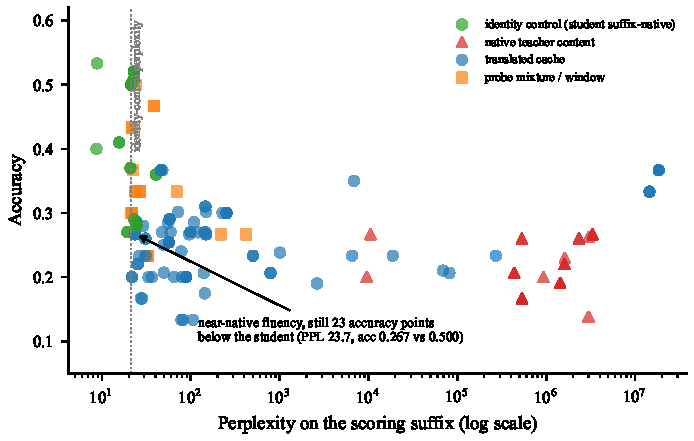
\includegraphics[width=0.68\columnwidth]{figures/fig4_ppl_acc_decoupling.pdf}
\caption{每个已记录方法与运行的打分后缀困惑度对准确率（对数尺度）。恒等对照——
即学生的后缀原生参照——位于左上角；翻译缓存散布在一条很宽的带上，其中包含一个
困惑度接近原生（$23.7$）却仍比学生的 $0.500$ 低 $23$ 个点的准确率的点。困惑度
并不按任务度量的方式给方法排序。}
\label{fig:decoupling}
\end{figure}

\begin{table}[h]
\centering
\caption{从教师状态恢复学生自身 $K$ 与 $V$ 的留出 $R^2$（逐（层，头）宏平均；
已记录处括号内为训练集数值）。这里的每个 $R^2$ 都是该映射器家族在固定的 20 个
校准上下文与 10 个留出上下文上的\emph{独立诊断重拟合}
（\texttt{scripts/measure\_reconstruction\_r2.py}），并不是产生
表~\ref{tab:main} 中 CHG 那一列的那个实例；因此配对是在家族之间，而不是在同一个
检查点与它自己的任务得分之间。更好的重建并不改变任务判定：联合 MLP 把仿射
映射器的值通道 $R^2$ 提高约 $49\%$（$0.323\to0.481$），而该家族仍然落在同一个
CHG 带内（表~\ref{tab:main}）。}
\label{tab:r2}
\resizebox{\columnwidth}{!}{%
\begin{tabular}{llccc}
\toprule
翻译器 & 源层组合 & $R^2_K$ & $R^2_V$ & 下游 CHG \\
\midrule
仿射逐头，$c{=}30$ & -- & 0.810 & 0.323 & $-0.138$ [$-0.312,+0.037$] \\
联合 MLP，$c{=}30$ & 全部层 & 0.854 (0.949) & 0.481 (0.647) & $-0.30$ 至 $-0.26$ \\
Top-$k$ 岭回归，$k{=}1,3,5$ & 取平均 & 0.822 / 0.787 / 0.762 & 0.317 / 0.248 / 0.182 & $-0.273$ / $-0.308$ / $-0.291$ \\
Top-$k$ 岭回归，$k{=}1,3,5$ & 拼接 & 0.826 / 0.858 / 0.864 & 0.326 / 0.419 / 0.428 & $-0.279$ / $-0.223$ / $-0.254$ \\
\bottomrule
\end{tabular}}
\end{table}

\begin{figure}[h]
\centering
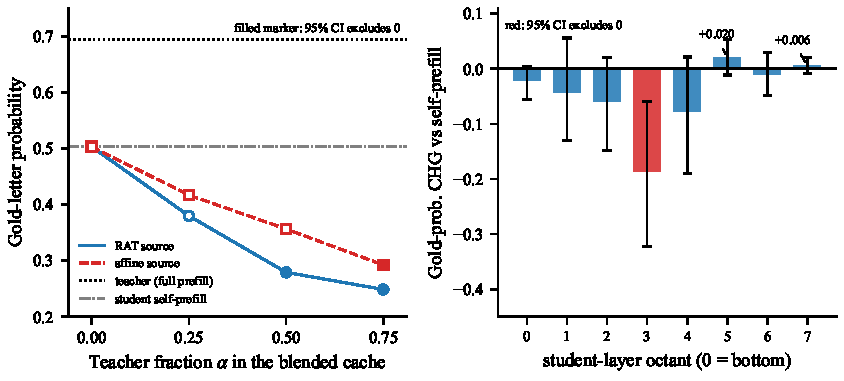
\includegraphics[width=0.95\columnwidth]{figures/fig3_oracle_probes.pdf}
\caption{主配对上的教师内容探针（$n{=}30$）。左：在两种翻译器下，当翻译内容替换
学生自身缓存时，三个混合占比下的金标字母概率（表~\ref{tab:probes}）。右：一次
探索性的仿射扫描，把八个学生层窗口之一替换为翻译内容，octant $0$ 为最底部；虚线
为学生自身的缓存。没有任何 octant 给出统计上成立的正面增益：最好的点估计为
$+0.020$ $[-0.012,+0.052]$。粗粒度的底/中/顶三分之一窗口在表~\ref{tab:probes}
中另行给出。}
\label{fig:probes}
\end{figure}

\begin{table}[h]
\centering
\caption{主配对上的教师内容探针，$n{=}30$。Gold 列为混合后的金标字母概率；CHG
相对学生自身 prefill。第一行是学生自身的缓存。两种翻译器一致认为：每个探针
要么退化要么中性，且替换顶部三分之一的层是中性的。}
\label{tab:probes}
\resizebox{\columnwidth}{!}{%
\setlength{\tabcolsep}{5pt}
\begin{tabular}{lcccc}
\toprule
探针 & Gold（RAT c30） & CHG（RAT c30） & Gold（仿射 c30） & CHG（仿射 c30） \\
\midrule
仅学生缓存（$\alpha{=}0$） & 0.503 & $+0.0001$ [$-0.0006, +0.0009$] & 0.503 & $+0.0001$ [$-0.0006, +0.0009$] \\
占比 $\alpha{=}0.25$ & 0.380 & $-0.123$ [$-0.258, +0.009$] & 0.417 & $-0.086$ [$-0.183, +0.003$] \\
占比 $\alpha{=}0.50$ & 0.279 & $-0.224$ [$-0.374, -0.077$] & 0.356 & $-0.147$ [$-0.322, +0.026$] \\
占比 $\alpha{=}0.75$ & 0.249 & $-0.254$ [$-0.423, -0.083$] & 0.292 & $-0.211$ [$-0.400, -0.012$] \\
窗口：顶部三分之一 & 0.502 & $-0.001$ [$-0.010, +0.010$] & 0.487 & $-0.016$ [$-0.120, +0.080$] \\
窗口：中部三分之一 & 0.265 & $-0.238$ [$-0.383, -0.106$] & 0.244 & $-0.259$ [$-0.413, -0.112$] \\
窗口：底部三分之一 & 0.224 & $-0.279$ [$-0.445, -0.105$] & 0.321 & $-0.182$ [$-0.306, -0.070$] \\
\bottomrule
\end{tabular}}
\end{table}

\textbf{族联合细节。} 确证性家族包含 RAT 翻译器下的三个混合占比与三个层窗口。
在 $10^4$ 次重采样上的联合 bootstrap 给出观测最大值 $-0.001$ 与 $95\%$ 上界估计
$+0.009$。

\section{与最接近已发表设计的非线性结果的关系}
\label{app:heo-mlp}

最接近的严格零 re-prefill 设计报告：在其线性映射退化剧烈的两条配对上，非线性
MLP 最多能恢复 $37$ 个 HellaSwag 保持率点~\citep{heo2026}。我们的梯度训练家族
没有帮助（表~\ref{tab:main}），而我们用的正是同一套四选一 HellaSwag/ARC 材料，
因此这两种读数必须对账。表~\ref{tab:heo-diff} 列出两组设定在四个维度上的差异。
仅凭已发表的数字，我们无法判断是哪一个维度承载了这一效应。两组设定的差别在于
报告的是什么量、在什么单位上：参考工作的非线性增益是在其线性映射退化剧烈的两条
配对上、以准确率保持率报告的，而我们的非线性各行是在固定留出样本上、以金标字母
概率评测的，校准规模也只有参考的五分之一。因此我们把 MLP 各行
读作关于本配置的证据，而不是对该结果的否证。

\begin{table}[h]
\centering
\caption{为什么非线性映射器在最接近的已发表设计中有效、在这里无效。只有前两行
在两组设定之间是对齐的。}
\label{tab:heo-diff}
\resizebox{\columnwidth}{!}{%
\begin{tabular}{lll}
\toprule
维度 & 本次审计 & 参考工作 \\
\midrule
配对条件 & 匹配 \kv{} 的 Qwen3 配对 & 匹配 \kv{} 的配对，三个家族共六条 \\
任务材料 & HellaSwag/ARC，四选一 & HellaSwag \\
报告量 & 金标字母概率变化，$95\%$ 置信区间 & 准确率保持率 \\
非线性增益的读取位置 & 每个家族的每次训练 & 线性映射失败的那两条配对 \\
校准规模 & $30$--$200$ 个样例（或 $100$ 条生成文本） & $500$ 条约 $1{,}024$ token 的序列 \\
\bottomrule
\end{tabular}}
\end{table}

\section{同期工作与负结果的作用域}
\label{app:concurrent}

近期工作提出了若干条让跨模型缓存复用成功的路线，它们的差别之一在于推理阶段是否
仍然保持严格零 re-prefill。正因为这一差别，我们的否定结论不能被读成对其中任何
一条路线的判断。

以接收方行为、而非缓存重建为训练目标的翻译器仍在严格零 re-prefill 下工作，并在
其测试的每一个配对上报告超越既有方法~\citep{cachelink2026}；用蒸馏训练的逐层
映射把拟合代价移到离线阶段，因此同样不违反该约束~\citep{kvlingo2026}；大模型
prefill、小模型解码的拆分方案让接收方直接读取翻译后的缓存~\citep{bridgekv2026}。
选择性重算走的是另一条路：它在自己判定的关键位置上花一小笔目标侧预填
~\citep{raracache2026}；稀疏迁移在固定 \kv{} 预算下界定被搬运的状态
~\citep{acct2026}；循环与卷积状态则承载了单靠注意力 \kv{} 无法承载的那部分交接
~\citep{latentport2026}。

因此，我们的否定结论适用于我们所测试的重建导向与架构先验翻译器，而不适用于所有
形式的功能性缓存搬运。真正可以沿用的是审计本身：三个判定门分别检查注入正确性、
对接收方自身预填的替代、以及能力增量，且不依赖译码器是如何得到的，因而可以原样
施加于上述每一类方法。实践上的推论是：任何翻译主张在报告保持率之前，应先说明它
走的是哪条路线、通过了哪个判定门。
\end{document}
